\documentclass[11pt]{article}
\usepackage{geometry, titlesec}
\usepackage[parfill]{parskip}
\usepackage[italicdiff]{physics}
\usepackage{amsfonts, amsthm}
\usepackage[cm]{fullpage}
\usepackage{fancyhdr}
\usepackage{enumitem}
\usepackage{xcolor, soul}
\usepackage{graphicx}
\usepackage[export]{adjustbox}
\usepackage{siunitx}
%\allowdisplaybreaks

\renewcommand{\thesubsection}{\thesection.\alph{subsection}}
\setenumerate[1]{label={(\alph*)}}

\makeatletter
\renewcommand*\env@cases[1][1.2]{%
  \let\@ifnextchar\new@ifnextchar
  \left\lbrace
  \def\arraystretch{#1}%
  \array{@{}l@{\quad}l@{}}%
}
\makeatother
 
\renewcommand{\footrulewidth}{.2pt}
%\setlist[enumerate]{leftmargin=*}
\pagestyle{fancy}
\fancyhf{}
\rhead{Physics 132-B}
\lhead{\textbf{Homework 5 Solutions}}
%\rhead{A--De Discussion}
\setlength{\headheight}{11pt}
\setlength{\headsep}{11pt}
\setlength{\footskip}{24pt}
\lfoot{\today}
\rfoot{\thepage}

\titleformat{\subsection}[runin]{\normalfont\large\bfseries}{\thesubsection}{1em}{}
\newcommand{\refeq}[1]{(\ref{#1})}

\newcommand{\beq}{\begin{equation*}}
\newcommand{\eeq}{\end{equation*}}

\newcommand{\beqn}{\begin{equation}}
\newcommand{\eeqn}{\end{equation}}

\newcommand{\blg}{\begin{align*}}
\newcommand{\elg}{\end{align*}}


\newenvironment{statement}
{
%    \color{gray}
    \ignorespaces
}
{
%    \smallskip
}

\newenvironment{problem}
{
    \color{darkgray}
    \ignorespaces
}

\newenvironment{solution}
{
    \paragraph{Solution.}
    \ignorespaces
}
{
    \bigskip
}

\renewcommand{\vec}[1]{\mathbf{#1}}
\renewcommand{\theequation}{\Alph{equation}}


\begin{document}

\newcommand{\Vab}{V_{ab}}
\newcommand{\cE}{\mathcal{E}}
\newcommand{\sicE}{\SI{12.0}{\volt}}
\newcommand{\sir}{\SI{0.40}{\ohm}}
\newcommand{\siP}{\SI{80.0}{\watt}}
	

\paragraph{Problem 25.58}
\begin{problem}
	A resistor with resistance $R$ is connected to a battery that has emf {\sicE} and internal resistance $r = \sir$.  For what two values of $R$ will the power in the resistor be {\siP}?
\end{problem}

\begin{solution}
	The power $P$ delivered to a resistor is
	\beqn \tag{25.18} \label{25.18}
		P = I^2 R,
	\eeqn
	where $I$ is the current through the resistor and $R$ its resistance.  We can find the current from
	\beqn \tag{25.17} \label{25.17}
		\Vab = \cE - I r,
	\eeqn
	where $\Vab$ is the voltage difference across the resistor, $\cE$ is the emf of the battery, and $r$ its internal resistance.  We also know that
	\beqn \tag{25.11} \label{25.11}
		\Vab = I R.
	\eeqn
	Substituting \refeq{25.11} into \refeq{25.17}, we get
	\beq
		IR = \cE - Ir
		\implies
		\cE = I (R + r)
		\implies
		I = \frac{\cE}{R + r}.
	\eeq
	Now we can substitute this result into \refeq{25.18} and solve for $R$:
	\begin{align*}
		P = \frac{\cE^2}{(R + r)^2} R
		&\implies
		\cE^2 R = P (R^2 + 2 R r + r^2)
		\implies
		0 = P R^2 + (2P r - \cE^2) R + P r^2 \\
		&\implies
		R = \frac{\cE^2 - 2 P r \pm \sqrt{(2P r - \cE^2)^2 - 4 P^2 r^2}}{2 P}
	\end{align*}
	Plugging in our numerical values for $r$, $P$, and $\cE$, and recalling that $\SI{1}{\watt} = \SI{1}{\square\volt\per\ohm}$, we get
	\begin{align*}
		R &= \frac{(\sicE)^2 - 2 (\siP) (\sir) \pm \sqrt{[2 (\siP) (\sir) - (\sicE)^2]^2 - 4 (\siP)^2 (\sir)^2}}{2 (\siP)} \\
		&= \frac{\SI{80.0}{\square\volt} - \pm \sqrt{(\SI{80}{\square\volt})^2 - (\SI{64}{\square\volt})}}{\SI{160}{\square\volt\per\ohm}}
		= \frac{\SI{80.0}{\square\volt} \pm \sqrt{\SI{2306}{\volt^4}}}{\SI{160}{\square\volt\per\ohm}}
		= \frac{80.0 \pm 48.0}{160} \,\si{\ohm}
		= (0.50 \pm 0.30) \,\si{\ohm} \\
		&= \begin{cases}
			{\color{blue} \SI{0.80}{\ohm}}, \\
			{\color{blue} \SI{0.20}{\ohm}}.
		\end{cases}
	\end{align*}
\end{solution}

\vfill
%\clearpage

\newcommand{\Iq}{I_1}
\newcommand{\Iw}{I_2}
\newcommand{\Ie}{I_3}

\begin{minipage}[l]{0.7\textwidth}
\paragraph{Exercise 26.26}
\begin{problem}
	In the circuit shown in \textbf{Fig.~E26.26}, find \medskip
	\begin{enumerate}
		\item the current in each branch, and \medskip
		\item the potential difference $\Vab$ of point $a$ relative to point $b$.
	\end{enumerate}
\end{problem}
\end{minipage}%
\hspace{0.05\textwidth}%
\begin{minipage}{0.25\textwidth}
	\center 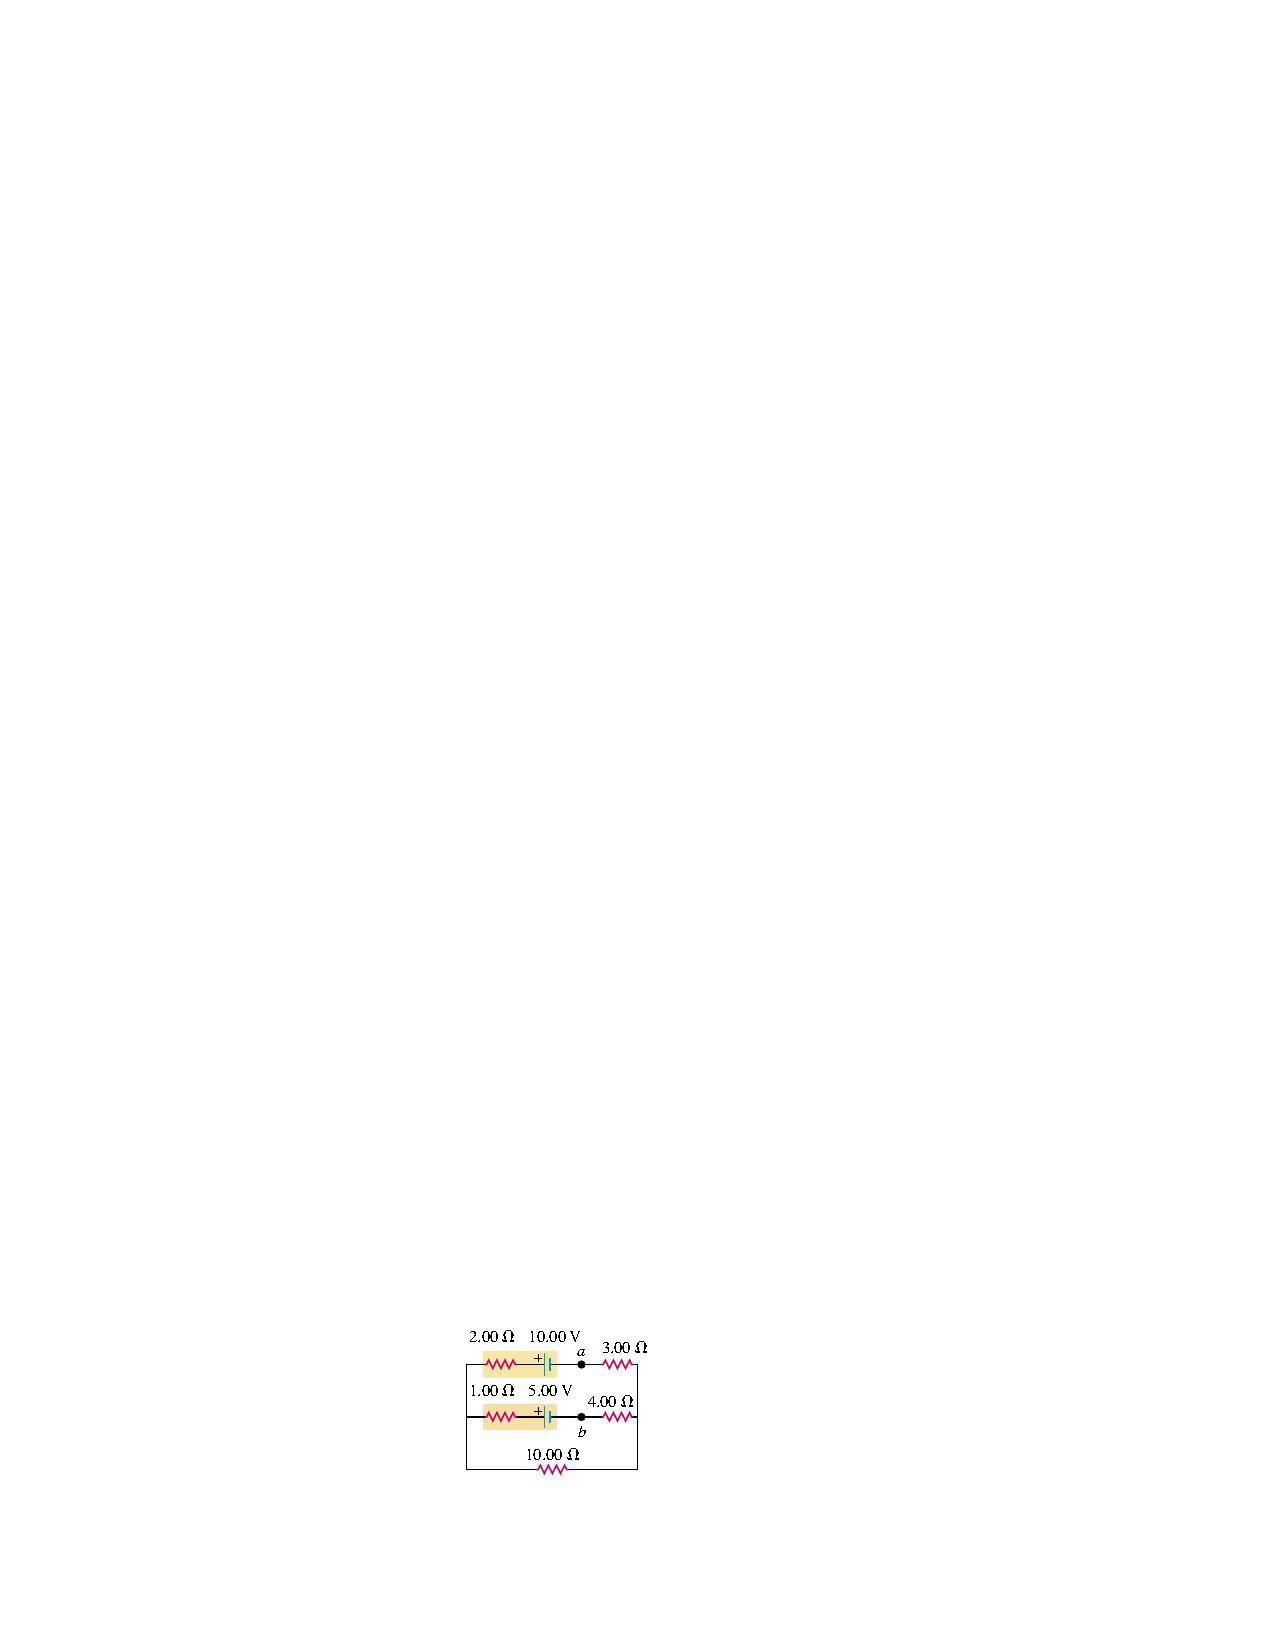
\includegraphics{E26-26}
	\center \textbf{Figure E26.26}
\end{minipage}

\vfill
\clearpage

%\begin{solution}
%	\begin{enumerate}
%		\item We need to use Kirchhoff's rules.  Since this circuit has more than one loop, we need to use both the junction rule,
%		\beqn \tag{26.5} \label{26.5}
%			\sum I = 0,
%		\eeqn
%		and the loop rule,
%		\beqn \tag{26.6} \label{26.6}
%			\sum V = 0.
%		\eeqn
%		Let's choose the current to be flowing to the right across the \SI{10.00}{\volt} battery, and start with the loop rule.  For the top loop, we have
%		\beqn 
%			0= \SI{10}{\volt} -\Iq (\SI{2}{\ohm}) - \Iq (\SI{1}{\ohm}) - \SI{5}{\volt} - \Iq (\SI{4}{\ohm}) - \Iq (\SI{3}{\ohm})
%			= \SI{5}{\volt} - \Iq (\SI{10}{\ohm})
%		\eeqn
%	\end{enumerate}
%\end{solution}

\begin{minipage}[l]{0.65\textwidth}
\paragraph{Exercise 26.29}
\begin{problem}
	In the circuit shown in \textbf{Fig.~E26.29} the batteries have negligible internal resistance and the meters are both idealized.  With the switch $S$ open, the voltmeter reads \SI{15.0}{\volt}. \medskip
	\begin{enumerate}
		\item Find the emf $\cE$ of the battery. \medskip
		\item What will the ammeter read when the switch is closed?
	\end{enumerate}
\end{problem}
\end{minipage}%
\hspace{0.05\textwidth}%
\begin{minipage}{0.3\textwidth}
	\center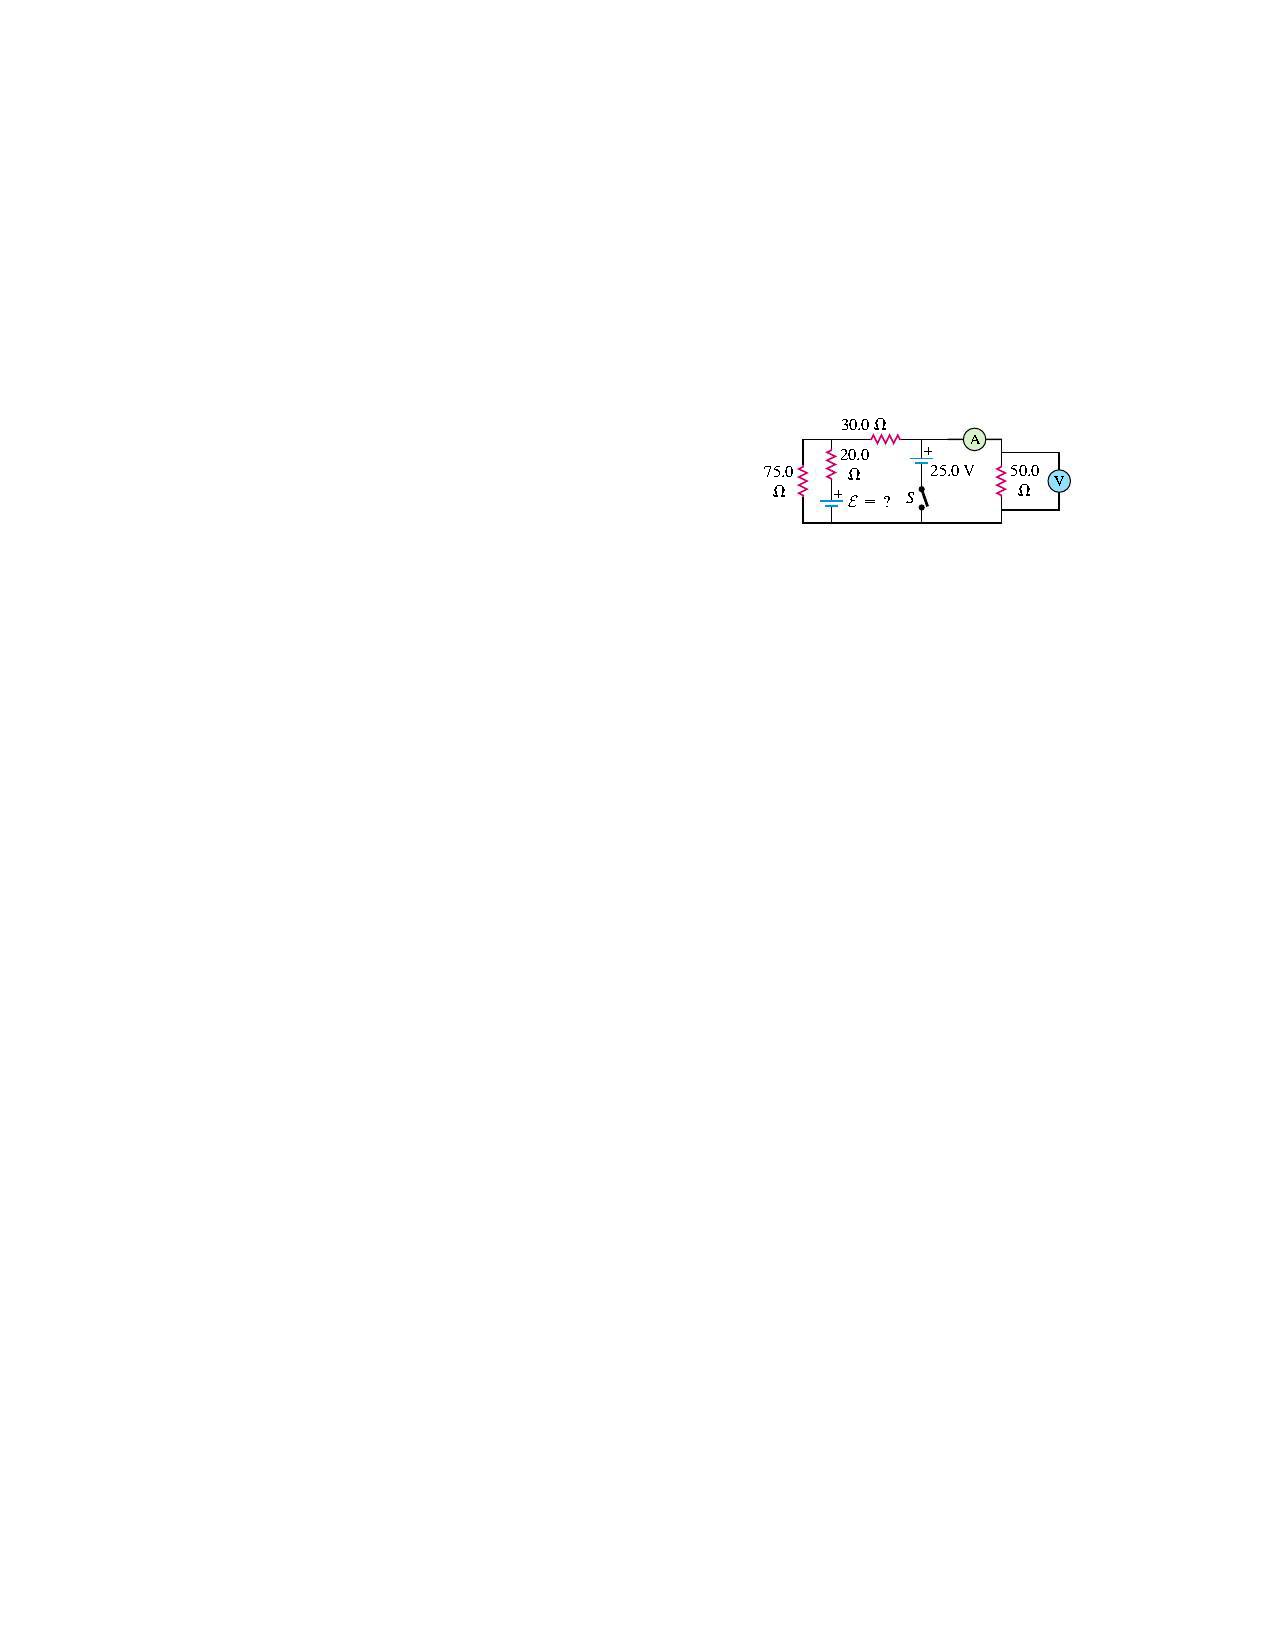
\includegraphics{E26-29}
	\center \textbf{Figure E26.29}
\end{minipage}

\vfill

\begin{minipage}[l]{0.75\textwidth}
\paragraph{Exercise 26.41}
\begin{problem}
	In the circuit shown in \textbf{Fig.~E26.41} both capacitors are initially charged to \SI{45.0}{\volt}. \medskip
	\begin{enumerate}
		\item How long after closing the switch $S$ will the potential across each capacitor be reduced to \SI{10.0}{\volt}, and \medskip
		\item what will be the current at that time? \medskip
	\end{enumerate}
\end{problem}
\end{minipage}%
\hspace{0.05\textwidth}%
\begin{minipage}{0.2\textwidth}
	\center 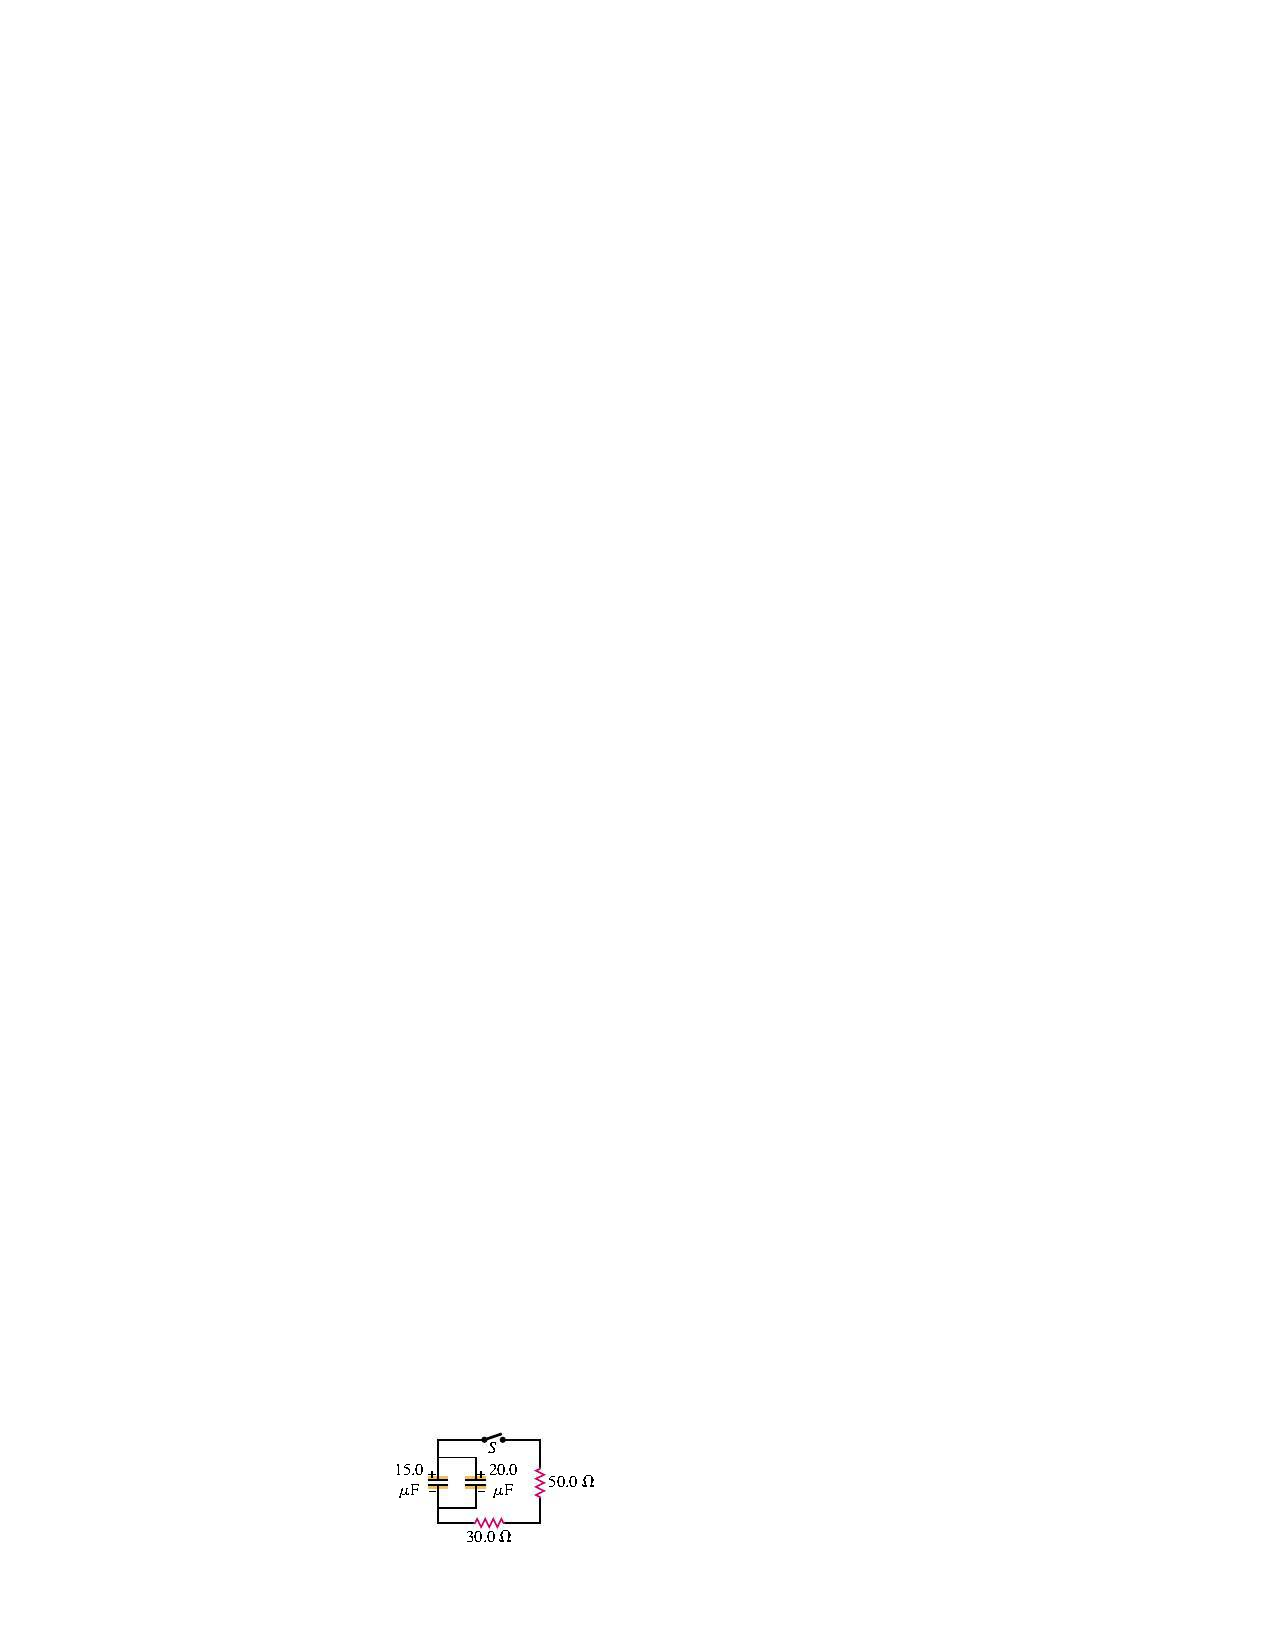
\includegraphics{E26-41}
	\center \textbf{Figure E26.41}
\end{minipage}

\vfill

\begin{minipage}[l]{0.55\textwidth}
\paragraph{Exercise 26.47}
\begin{problem}
	In the circuit shown in \textbf{Fig.~E26.47} the capacitors are initially uncharged, the battery has no internal resistance, and the ammeter is idealized.  Find the ammeter reading \medskip
	\begin{enumerate}
		\item just after the switch $S$ is closed, and \medskip
		\item after $S$ has been closed for a very long time.
	\end{enumerate}
\end{problem}
\end{minipage}%
\hspace{0.05\textwidth}%
\begin{minipage}{0.4\textwidth}
	\center 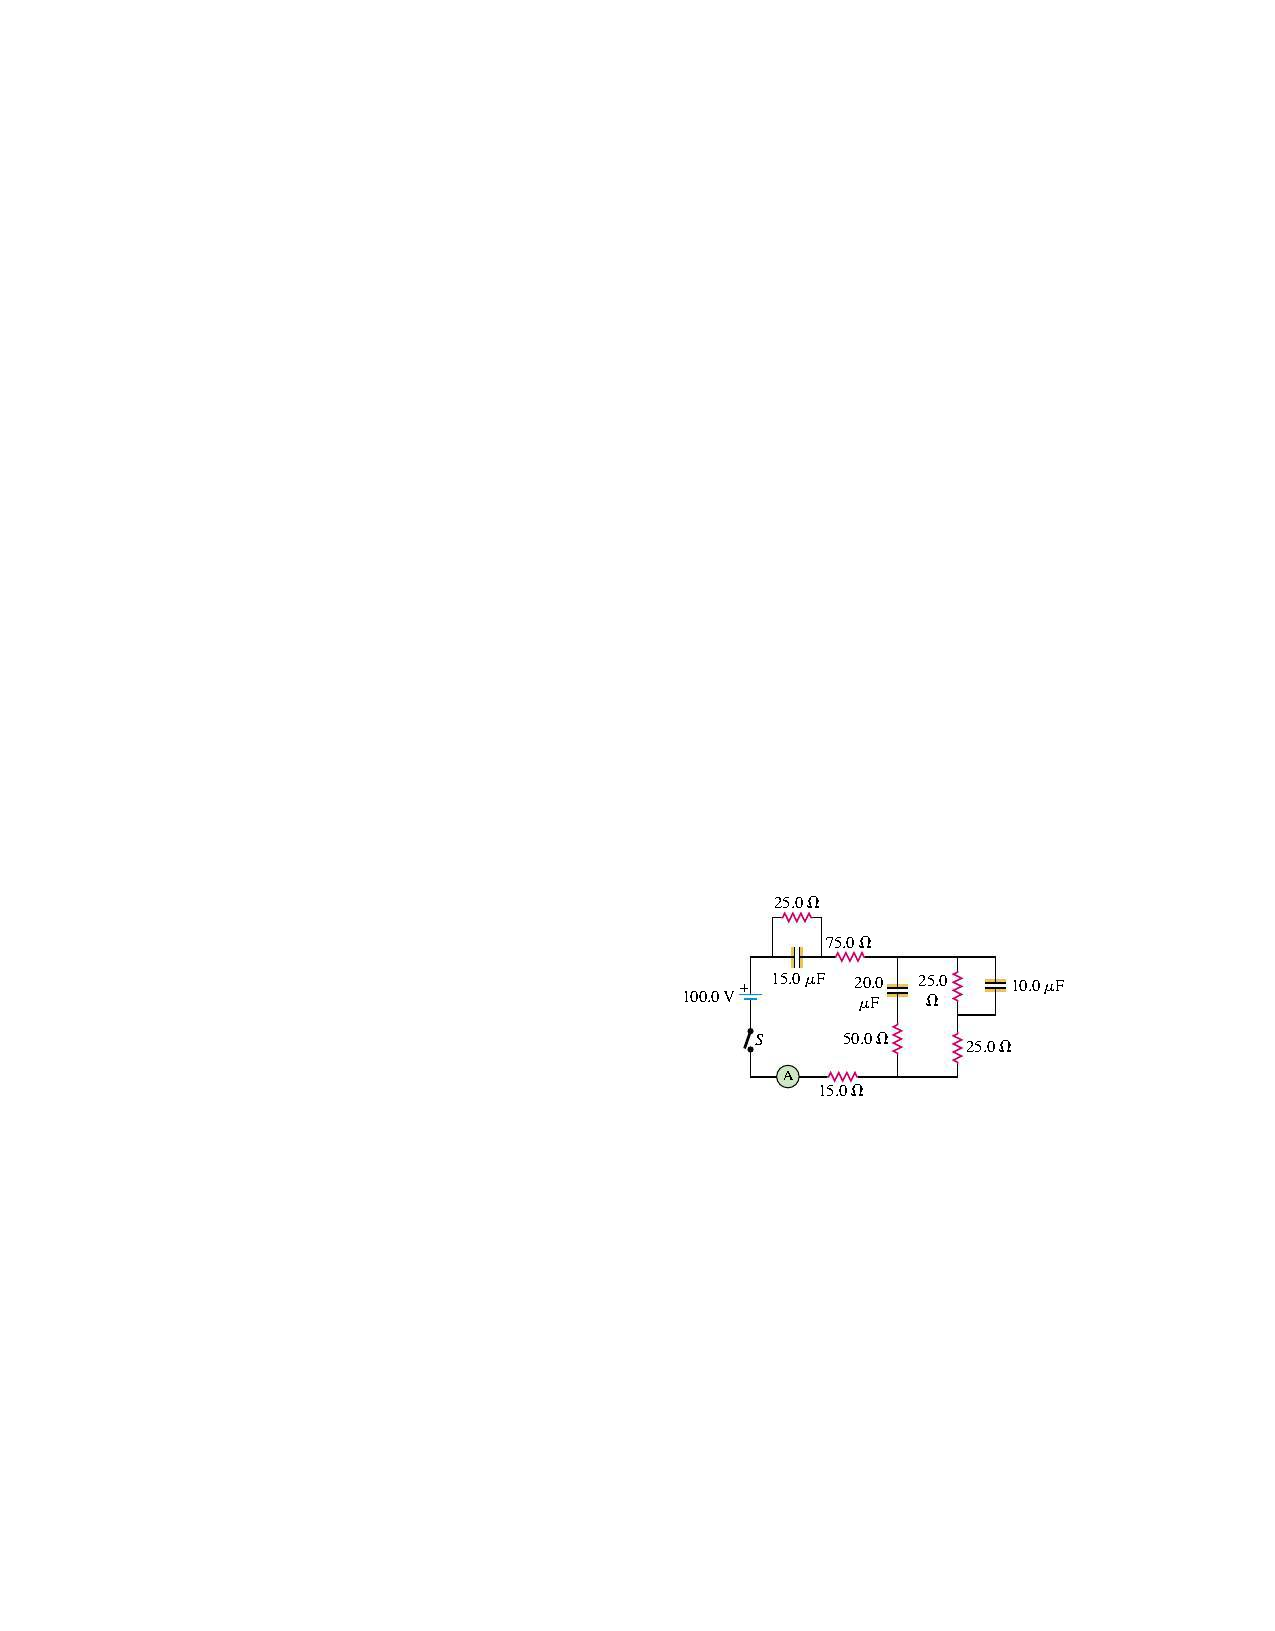
\includegraphics{E26-47}
	\center \textbf{Figure E26.47}
\end{minipage}

\vfill


\newcommand{\PcE}{P_\cE}
\newcommand{\dt}{\dd{t}}
\newcommand{\PR}{P_R}

\paragraph{Problem 26.53}
\begin{problem}
	A capacitor with capacitance $C$ is connected in series to a resistor of resistance $R$ and a battery with emf $\cE$.  The circuit is completed at time $t = 0$.
	\begin{enumerate}
		\item In terms of $\cE$, $R$, and $C$, how much energy is stored in the capacitor when it is fully charged?
		\item The power output of the battery is $\PcE = \cE i$, with $i$ given by Eq.~(26.13).  The electrical energy supplied in an infinitesimal time $\dt$ is $\PcE \dt$.  Integrate from $t = 0$ to $t \to \infty$ to find the total energy supplied by the battery.
		\item The rate of consumption of electrical energy in the resistor is $\PR = i^2 R$.  In an infinitesimal time interval $\dt$, the amount of electrical energy consumed by the resistor is $\PR \dt$.  Integrate from $t = 0$ to $t \to \infty$ to find the total energy consumed by the resistor.
		\item What fraction of the total energy supplied by the battery is stored in the capacitor?  What fraction is consumed in the resistor?
	\end{enumerate}
\end{problem}

\vfill

\begin{minipage}[l]{0.7\textwidth}
\paragraph{Problem 26.59}
\begin{problem}
	Calculate the currents $\Iq$, $\Iw$, and $\Ie$ indicated in the circuit diagram shown in \textbf{Fig.~P26.59}.
\end{problem}
\end{minipage}%
\hspace{0.05\textwidth}%
\begin{minipage}{0.25\textwidth}
	\center 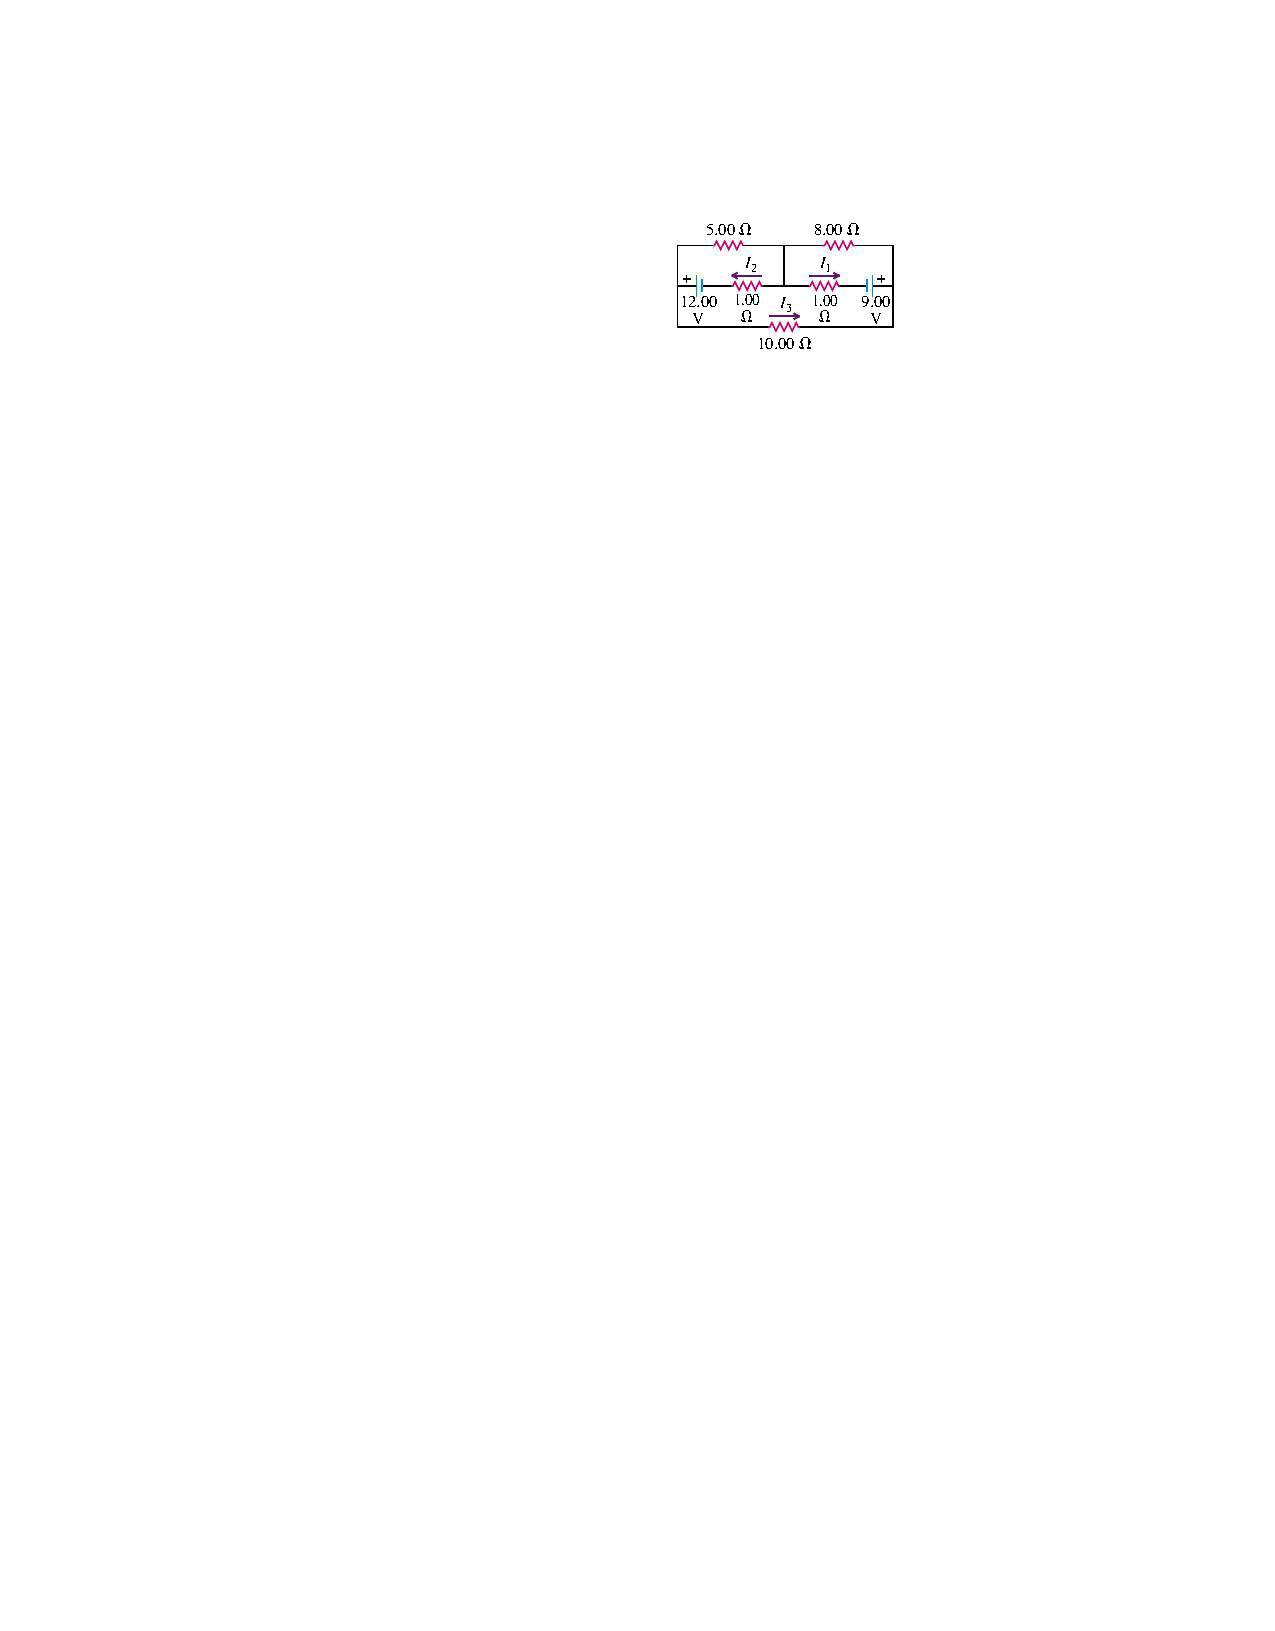
\includegraphics{P26-59}
	\center \textbf{Figure P26.59}
\end{minipage}

\vfill


\end{document}